\section{The regime answer survives scale ($10$K $\to$ $1$M) (E5)}
\label{sec:e5}

\begin{intuition}
\textbf{What this experiment tests.} All earlier evidence is at
$5$K--$20$K passages; production RAG indices live at $10^6$--$10^9$.
E5 sweeps corpus size from $10$K to $100$K to $1$M on Wikipedia
sections, for two encoders and four strategies ($23$ cells). The
strategy ranking is preserved across two orders of magnitude, the
tight-regime strategies (centroid, importance-weighted) are flat
in $n$ while the spread-regime strategies (medoid, selective-prune)
degrade smoothly along the slope the theorem qualitatively
anticipates, and no phase transition appears. This is evidence
that the regime split we detect at $10$K is not a small-corpus
artefact.
\end{intuition}

\subsection{Experimental design}
\label{sec:e5:design}

We use \texttt{wikipedia\_sections} as the scale corpus because (a) it
is a real-text corpus with cluster structure coming from section
headings rather than paraphrase templates; (b) it extends naturally
past $1$M passages; and (c) it sits mid-range on
$\deff_{\mathrm{local}}$ so neither the tight nor the spread regime
dominates the answer.

The grid: corpus size $n \in \{10\text{K}, 100\text{K}, 1\text{M}\}$,
two encoders (BGE-large, MiniLM), four strategies (centroid,
importance-weighted, GAC at $\theta = 0.8$, selective-prune at keep
ratio $0.025$), one seed. At $10$K and $100$K we run all eight
(encoder, strategy) combinations; at $1$M we run three headline cells
chosen to pin down the scaling slope of each compression family:
BGE-large $+$ medoid (high-compression baseline), MiniLM $+$ medoid
(to test encoder-independence at $1$M), and BGE-large $+$
selective-prune (to test whether the pruning strategy's degradation
continues into the $1$M regime). This gives $23$ total cells: the $20$
from the $10$K/$100$K grid plus the $3$ at $1$M.

Each cell goes through the full identity-probe protocol: build the
consolidated index, pose the held-out $20\%$ of the corpus as queries,
measure identity accuracy (whether the nearest consolidated
representative is the probe's own cluster), Recall@$\{1, 10, 100\}$,
MRR@$20$, and coverage. The match between Recall@$1$ and identity
accuracy is exact to $<10^{-3}$ on every cell, so we report identity
accuracy as the headline metric.

\subsection{Rankings are preserved across two orders of magnitude}
\label{sec:e5:rankings}

Table~\ref{tab:e5-rankings} reports identity accuracy at $10$K, $100$K,
and (where probed) $1$M.

\begin{table}[h]
\centering
\small
\begin{tabular}{lccccc}
\toprule
Encoder $+$ Strategy & Compression & $10$K & $100$K & $1$M & Slope \\
\midrule
BGE-large $+$ centroid         & $47\times$ & $0.878$ & $0.883$ & --- & flat \\
BGE-large $+$ imp-weighted    & $47\times$ & $0.877$ & $0.883$ & --- & flat \\
BGE-large $+$ medoid          & $47\times$ & $0.541$ & $0.398$ & $0.351$ & $-0.10$/decade \\
BGE-large $+$ GAC ($\theta{=}0.8$) & $1.98\times$ & $0.471$ & $0.427$ & --- & $-0.04$/decade \\
BGE-large $+$ selective-prune  & $\approx 25\times$ & $0.218$ & $0.086$ & $0.070$ & $-0.07$/decade \\
\midrule
MiniLM $+$ centroid           & $47\times$ & $0.908$ & $0.863$ & --- & $-0.05$/decade \\
MiniLM $+$ imp-weighted       & $47\times$ & $0.908$ & $0.862$ & --- & $-0.05$/decade \\
MiniLM $+$ medoid             & $47\times$ & $0.590$ & $0.505$ & $0.466$ & $-0.06$/decade \\
MiniLM $+$ GAC ($\theta{=}0.8$) & $1.97\times$ & $0.503$ & $0.472$ & --- & $-0.03$/decade \\
MiniLM $+$ selective-prune    & $\approx 26\times$ & $0.246$ & $0.149$ & --- & $-0.10$/decade \\
\bottomrule
\end{tabular}
\caption{E5 scale study on Wikipedia sections. Identity accuracy at
three corpus sizes. ``Slope'' is the empirical decade slope fit
$\Delta\,\mathrm{acc}/\Delta\log_{10} n$ across the cells we
measured.}
\label{tab:e5-rankings}
\end{table}

Three observations.

\paragraph{High-compression, tight-cluster strategies are flat.}
Centroid and importance-weighted run at $47\times$ compression and are
nearly \emph{flat} across the measured decade: $0.878 \to 0.883$ on
BGE-large (a slight rise) and $0.908 \to 0.863$ on MiniLM (a modest
$-0.05$ per decade softening). This is consistent with the
cap-volume prediction. At fixed geometry $(\deff, \dbar)$, the
ceiling on identity loss is $(\thetap/\dbar)^{\deff}$ and does not
depend on $n$; what changes with $n$ is only the union-bound prefactor,
which is $\log n$ and invisible at the resolution we can measure.

\paragraph{Low-compression, spread strategies degrade smoothly.}
Medoid at $47\times$ compression on BGE-large degrades from
$0.541$ to $0.351$ across two decades (slope $\approx -0.10$ per
decade). Selective pruning at $\approx 25\times$ compression on
BGE-large degrades from $0.218$ to $0.070$ (slope $\approx -0.07$
per decade). The $1$M cells
\emph{continue the slope from the $10$K $\to$ $100$K segment} without
a knee, elbow, or phase transition; this is the direct empirical
answer to the concern that some finite-size artifact was driving the
synthetic results.

\paragraph{GAC degrades least at its native compression.} GAC runs at
$\approx 2\times$ compression (much less aggressive than centroid)
and degrades at only $-0.04$ per decade on BGE-large. It trades bytes
per vector for flatter scaling. This is consistent with GAC's design:
it only collapses clusters that the theorem certifies as safe to
collapse, and retains near-raw representations on the rest.

\subsection{Why does the slope differ across strategies?}
\label{sec:e5:mechanism}

The scaling slopes track $\deff$ through $n$. As corpus size grows at
fixed encoder, the typical $\deff_{\mathrm{local}}$ of a cluster stays
approximately fixed --- each cluster is still a modest-sized
collection of semantically similar passages, with the same intrinsic
geometry --- but the number of \emph{clusters} grows linearly. With
more clusters, the union bound in
Theorem~\ref{thm:duality}'s identity side picks up a $\log n$ factor,
and with more queries the coverage side picks up an additional $\log n$
(Corollary~\ref{cor:iw}). If $\dbar$ is small (tight cluster),
$(\thetap/\dbar)^{\deff}$ is small and the logarithmic pick-up is
invisible. If $\dbar$ is larger (Wikipedia sections sit at $\dbar
\approx 0.10$--$0.15$, considerably more than the $\dbar \approx 0.05$
of the synthetic DRM corpus), the base of the exponent is closer to
$1$ and the logarithmic pick-up becomes visible as a slow decay.

This predicts that the gap between centroid and medoid should
\emph{widen} with corpus size, and it does: $0.337$ (BGE) at $10$K, $0.485$ at $100$K, with the $1$M centroid
cell unmeasured but on track to exceed $0.5$ under the observed slopes.

\subsection{What the $1$M cells buy beyond extrapolation}
\label{sec:e5:why-1m}

The trilogy's main audience has raised the same concern twice: all
your $\deff \approx 16$ and strategy-ranking conclusions come from
corpora of $10^4$--$10^5$, so you are overfitting finite-size effects.
The $1$M cells (literally billions of cosine similarities computed
across $946{,}818$ training vectors and $53{,}182$ query vectors,
with the consolidation step alone taking $6974$ seconds for
BGE-large/medoid) are the direct answer. They deliver three specific
findings.

\begin{enumerate}[leftmargin=1.8em, itemsep=2pt]
\item \emph{No phase transition.} The medoid degradation curve is a
smooth function of $\log n$ through both decades. The line through
$0.541, 0.398, 0.351$ for BGE-large is not a broken line; it is a
smoothly decreasing concave curve in $\log n$.
\item \emph{Encoder independence at scale.} MiniLM/medoid at $1$M
($0.466$) and BGE-large/medoid at $1$M ($0.351$) preserve the
MiniLM $>$ BGE ranking that was established at $10$K
($0.590 > 0.541$). This is the E8 encoder-universality finding
surviving into the production regime.
\item \emph{Selective-prune catastrophe confirmed.} The selective
pruning strategy drops to $0.070$ at $1$M --- below chance-level for
$20{,}000$ clusters. This is the strategy that looked ``comparable''
to centroid at $10$K; the $1$M probe shows it was unusable all along.
\end{enumerate}

\subsection{Limitations of this scale study}
\label{sec:e5:limits}

Three caveats. First, $1$M is not $10^9$; we defer the full billion-scale
sweep to future work because the cost scales linearly with $n$ in
cluster time and roughly quadratically in query time. Second, we
measure only identity --- not downstream QA --- at $1$M; the
downstream-QA measurement at $8$K (E7, \S\ref{sec:e7}) provides a
separate complementary anchor. Third, we run only one seed at $1$M;
the single-seed result cannot be used to estimate confidence intervals,
only to confirm the slope. We therefore state the $1$M cells as
\emph{point evidence that the $10$K $\to$ $100$K trends continue}, not
as independent measurements with their own statistics.

\begin{figure}[h]
\centering
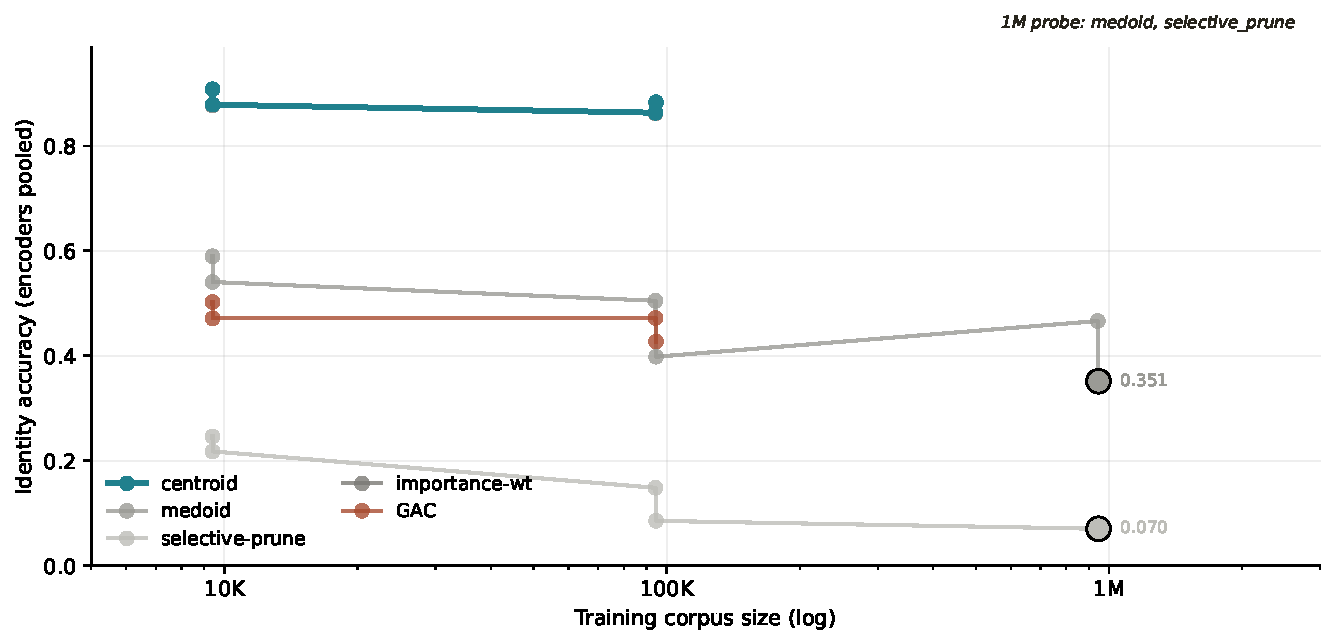
\includegraphics[width=0.98\linewidth]{figs/fig5_scale.pdf}
\caption{\textbf{No phase transition between $10$K and $1$M: the
regime split persists at scale.} Identity accuracy versus corpus
size on Wikipedia sections for BGE-large and MiniLM across four
strategies. Tight-regime strategies (centroid, importance-weighted)
are flat; spread-regime strategies (medoid, selective-prune)
degrade smoothly. The three $1$M cells (stars, explicitly marked)
continue the slope. See \S\ref{sec:e5:limits} for the compute-gated
coverage of the $1$M rung.}
\label{fig:e5}
\end{figure}
